\chapter{Evaluierung}\label{kap:eval}

In diesem Kapitel wird die Auswertung der 
Ergebnisse der trainierten Modelle beschrieben.

Dafür werden im ersten Abschnitt zunächst die Metriken 
erklärt, anhand derer die Evaluierung erfolgte. 

Im zweiten Abschnitt werden die beiden verwendeten Object 
detection Modelle Single Shot Detector (SSD)
und Faster R-CNN hinsichtlich dieser Metriken
sowie anhand von
Inferenzergebnissen verglichen.

Der dritte Abschnitt beschreibt Methoden, mit denen 
die Ergebnisse des Faster R-CNN optimiert werden konnten.

Im vierten Abschnitt werden die Modelle hinsichtlich 
der Inferenzzeit miteinander verglichen.


\section{Evaluierungsmetriken}\label{sec:metricen}

Zur Messung der Genauigkeit der Object detection Modelle 
wurde die \textit{Mean Average Precision} (mAP) verwendet.
Diese bezieht sowohl Klassifikations-, als auch
Lokalisierungsgenauigkeit mit ein und
lässt sich aus den folgenden Werten berechnen.

\begin{itemize}
  \item \textit{True Positive (TP)}:
  Das Modell hat richtig das Vorhandensein eines Objekts geschätzt
  \item \textit{True Negative (TN)}:
  Das Modell hat richtig die Abwesenheit eines Objekts geschätzt
  \item \textit{False Positive (FP)}:
  Das Modell hat fälschlicherweise das Vorhandensein eines Objekts
  geschätzt
  \item \textit{False Negative (FN)}:
  Das Modell hat fälschlicherweise die Abwesenheit eines Objekts
  geschätzt
\end{itemize}

Die Festlegung für \textit{True Positive} Werte wird dabei über die
sogenannte \textit{Intersection over Union} (IoU) ermittelt,
welche in Abbildung \ref{fig:iou} dargestellt ist.


Diese ist durch den Überlappungsgrad der im Label definierten
\textit{Ground-Truth}-Bounding-Box und der geschätzten Bounding-Box
bezogen auf den Gesamtbereich, den die beiden Boxen einschließen,
definiert.

Ist der Überlappungsgrad größer als ein definierter Threshold,
der häufig bei 50\% liegt, gilt die Schätzung als
\textit{True Positive}, andernfalls als \textit{False Positive}.

\newcommand\MyBox[2]{
  \fbox{\lower0.75cm
    \vbox to 1.7cm{\vfil
      \hbox to 1.7cm{\hfil\parbox{1.4cm}{#1\\#2}\hfil}
      \vfil}
  }
}
\noindent
\renewcommand\arraystretch{1.5}
\setlength\tabcolsep{0pt}

\begin{minipage}{\textwidth}
    \begin{minipage}[b]{0.49\textwidth}
      \centering
      \def\svgwidth{0.8\textwidth}
      \input{Bilder/IoU_formula.pdf_tex}
      \captionof{figure}{Intersection over Union}
      \label{fig:iou}
  \end{minipage}
    \hfill
    \begin{minipage}[b]{0.49\textwidth}
      \centering
      \begin{tabular}{c >{\bfseries}r @{\hspace{0.7em}}c @{\hspace{0.4em}}c @{\hspace{0.7em}}l}
        \multirow{10}{*}{\rotatebox{90}{\parbox{2.5cm}{\bfseries\centering Tatsächlicher Wert}}} & 
          & \multicolumn{2}{c}{\bfseries Geschätzter Wert} & \\
        & & \bfseries p & \bfseries n & \bfseries\\
        & p$'$ & \MyBox{True}{Positive} & \MyBox{False}{Negative}\\[2.4em]
        & n$'$ & \MyBox{False}{Positive} & \MyBox{True}{Negative} \\
      \end{tabular}
        \captionof{figure}{Confusion Matrix}
        \label{fig:confusion_matrix}
    \end{minipage}
\end{minipage}
\vspace{1cm}

Anhand dieser in der \textit{Confusion Matrix} (Abbildung
\ref{fig:confusion_matrix}) dargestellen Werte
lassen sich die Metriken \textit{Precision} und
\textit{Recall} berechnen.

Der \textit{Recall} ist dabei durch das Verhältnis der
richtig gefundenen zu allen sich im Bild befindenden Objekten
definiert, was sich auch durch das, in Gleichung \ref{eq:recall}
gezeigte Verhältnis von True Positive 
und False Positive, darstellen lässt.
\vspace{0.5cm}

\begin{equation}
  \label{eq:recall}
  Recall = \frac{TP}{TP + FN}
\end{equation}
\vspace{0.5cm}

Im Gegensatz zum \textit{Recall}, der die Trefferquote
des Modells angibt, gibt die \textit{Precision} die Genauigkeit
an, mit der die Objekte gefunden wurden.
Definiert ist diese \textit{Precision} durch das 
Verhältnis der richtigen Schätzungen bezogen
auf alle gemachten Schätzungen,
was auch durch das, in Gleichung \ref{eq:precision}
dargestellte, Verhältnis von True Positives und False Positives 
ausgedrückt werden kann.
\vspace{0.5cm}

\begin{equation}
  \label{eq:precision}
  Precision = \frac{TP}{TP + FP}
\end{equation}
\vspace{0.5cm}

Werden für eine Klasse alle \textit{Precision}-Werte
über dem \textit{Recall} abgebildet, 
ergibt sich eine abnehmende Kurve, 
dessen Flächeninhalt, wie in Gleichung 
\ref{eq:ap} dargestellt, die durchschnittliche 
\textit{Precision} für diese Klasse darstellt.

Wird die durchschnittliche 
\textit{Precision} für alle Klassen gebildet und 
im Mittel genommen, erhält man die in 
Gleichung \ref{eq:map} dargestellte,
\textit{mean Average Precision} (mAP).

\vspace{0.5cm}
\begin{equation}
  \label{eq:ap}
  \text{Average Precision} = \sum Precision(Recall)
\end{equation}
\vspace{0.5cm}
\begin{equation}
  \label{eq:map}
  mAP = \frac{1}{N} \sum \text{Average Precision}
\end{equation}
\vspace{0.5cm}


% \subsection*{Fehlerfunktion (Loss)}
% Die Fehlerfunktion setzet sich aus einem Lokalisierungs- und einem 
% Klassifikationsfehler zusammen. 
% Die Lokalisierung erfolgt über eine Lineare Regression zur 
% Annäherung der Bounding Boxes and die richtigen Koordinaten.



%----------------- SECTION: validtaion ---------------------
\section{Vergleich der Modelle}\label{sec:model_vergleich}

In diesem Abschnitt geht es um die Auswertung 
der Evaluierungsergebnisse der beiden für das Training 
verwendeten Object-detection-Architekturen Single
Shot Detector (SSD) und Faster R-CNN.


\subsection{Evaluierung}

Die im Folgenden dargestellten Ergebnisse beziehen sich auf 
den Validierungsanteil des für das Training verwendeten
\textit{Open Images} Datensatzes.

Die Berechnung der Evaluierungsergebnisse
anhand der in Abschnitt
\ref{sec:metricen} erläuterten Metriken, sowie 
eine visualisierte Darstellung 
des Trainingsverlaufs, erfolgte
über das Evaluierungstool \textit{TensorBoard}.

Das Training wurde für alle drei Modelle
sowohl für den originalen, als auch für den
augmentierten Datensatz durchgeführt.

\vspace{0.5cm}
\begin{table}[H]
  \centering
  \begin{tabular}{m{0.25\textwidth}m{0.3\textwidth}|m{0.15\textwidth}<{\centering}m{0.15\textwidth}<{\centering}}
  \hline
  Model                                                              & Optimierung                                                                   & mAP                                                        & Loss                                                       \\ \hline\hline
  SSD + MobilenetV2                                                  & \begin{tabular}[c]{@{}l@{}}ohne Augmentierung\\mit Augmentierung\end{tabular}                  & \begin{tabular}[c]{@{}l@{}}0,62\\ 0,61\end{tabular}        & \begin{tabular}[c]{@{}l@{}}3,56\\ 3,50\end{tabular}        \\ \hline
  SSD + InceptionV2                                                  & \begin{tabular}[c]{@{}l@{}}ohne Augmentierung\\mit Augmentierung\end{tabular}                  & \begin{tabular}[c]{@{}l@{}}0,65\\ 0,62\end{tabular}        & \begin{tabular}[c]{@{}l@{}}3,86\\ 3,71\end{tabular}        \\ \hline
  \begin{tabular}[c]{@{}l@{}}Faster R-CNN\\ +InceptionV2\end{tabular} & \begin{tabular}[c]{@{}l@{}}ohne Augmentierung\\mit Augmentierung\\ Early Stopping\end{tabular} & \begin{tabular}[c]{@{}l@{}}0,67\\ 0,69\\ 0,67\end{tabular} & \begin{tabular}[c]{@{}l@{}}0,82\\ 0,67\\ 0,69\end{tabular} \\ \hline
  \end{tabular}
  \caption{Trainingsergebnisse: SSD und Faster R-CNN}
  \label{table:model_vgl}
\end{table}
\vspace{0.5cm}

Anhand der in Tabelle \ref{table:model_vgl} dargestellten 
Ergebnisse ist zu erkennen, dass sich mit dem zweistufigen 
Faster R-CNN bessere Ergebnisse als mit dem einstufigen
SSD erzielen ließen.
Der Unterschied ist besonders deutlich anhand des Loss-Wertes 
festzustellen.

Des Weiteren wurden bei den SSD Konfigurationen, mit dem 
InceptionV2
als Basis \Gls{cnn}, bessere Ergebnisse erreicht, als mit dem 
MobilenetV2.

Bei allen Modellen war durch die Augmentierung des 
Datensatzes eine Verbesserung des Loss-Wertes festzustellen, 
da auf diese Weise auftretendes \Gls{overfitting} reduziert
oder verhindert werden konnte.

Bei den SSD-Architekturen führte die Augmentierung
jedoch auch zu einer Verringerung des mAP-Wertes, 
was auf die weniger komplexe Modellstruktur zurückzuführen sein kann.

Je mehr Parameter einem Modell zur Verfügung stehen, desto besser kann 
es sich an die Trainingsdaten anpassen, desto eher findet jedoch
auch \Gls{overfitting} statt.
Dieser Zusammenhang hat sich deutlich bei dem Faster R-CNN 
Modell bemerkbar gemacht.

Der Plot in Abbildung \ref{plot:loss} zeigt den Trainingsverlauf
der verschiedenen Faster R-CNN-Trainingskonfigurationen
anhand der Loss-Kurve.

Für das Training mit dem originalen Datensatz nimmt der Loss-Wert
nach ca. 100k Iterationen wieder zu, wohingegen der Loss beim Training 
mit augmentierten Datensatz den Wert weitestgehend beibehält.

\textit{Early Stopping} war ein weiterer Ansatz, das 
\Gls{overfitting} beim Faster-R-CNN-Modell zu verhindern.
Dafür wurde das Training vor der Wiederzunahme des Loss-Wertes 
abgebrochen.

Anhand der Loss-Kurve im Plot in Abbildung \ref{plot:loss} 
ist zu erkennen, dass sich dadurch der gleiche
Wert wie durch die Augmentierung erreichen ließ.
Jedoch konnte der mAP, wie im Plot in Abbildung \ref{plot:mAP}
zu erkennen ist, durch das frühzeitige Stoppen des 
Trainings, seinen möglichen Endwert nicht erreichen.


\vspace{0.5cm}
\begin{figure}[H]
\begin{minipage}{0.5\textwidth}
  \centering
  \def\svgwidth{0.95\textwidth}
  \input{Bilder/plots/overfitting_kein_early_aug_mAP.pdf_tex}
  \captionof{figure}{Trainingsverläufe: Faster\\R-CNN, mAP}
  \label{plot:mAP}
\end{minipage}
\begin{minipage}{0.5\textwidth}
  \centering
  \def\svgwidth{0.95\textwidth}
  \input{Bilder/plots/overfitting_kein_early_aug_loss.pdf_tex}
  \captionof{figure}{Trainingsverläufe: Faster\\R-CNN, Loss}
  \label{plot:loss}
\end{minipage}
\end{figure}

% Legende: Overfitting
\begin{table}[htb]
  \centering
  \begin{tabular}{m{0.1\textwidth}<{\centering}
                  m{0.2\textwidth}<{\centering}
                  m{0.2\textwidth}<{\centering}}
      $\color[HTML]{FF7043}\medbullet$  Ohne 
    & $\color[HTML]{0077BB}\medbullet$  Early Stopping 
    & $\color[HTML]{CC3311}\medbullet$  Augmentierung
  \end{tabular}    
\end{table}

% colors
% orange: FF7043
% blue  : 0077BB
% red   : CC3311

Daraus ließe sich schließen, dass die Augmentierung das 
bessere Vorgehen zur Vermeidung von \Gls{overfitting} ist.
Um herauszufinden, ob sich diese Annahme bestätigt 
und wie sehr sich die unterschiedlichen Ergebnisse
zwischen SSD und Faster R-CNN in der praktischen Anwendung
bemerkbar machen, wurde die Inferenz der
trainierten Modelle testweise auf verschiedene Bilder
ausgeführt.


%----------------- SECTION: Test Inferenz ---------------------
\subsection{Test Inferenz}\label{sec:test_inferenz}

Um die Inferenz ausführen zu 
können, wurden die trainierten Modelle, wie in Abschnitt
\ref{sec:inferenz} beschrieben, 
in die \textit{Intermediate Representation} konvertiert 
und anschließend mithilfe der \textit{Inference Engine} auf 
dem \textit{Neural Compute Stick 2} inferiert.

Dafür wurden zunächst die Bilder aus dem Testset des
\textit{Open Images} Datensatzes verwendet. Da diese jedoch 
sehr ähnlich zu den Trainingsdaten sind, wurden 
auch Bilder aus anderen Quellen inferiert.
Als weiterer Testdatensatz wurden, zum einen Teile des
\textit{iWildCam 2019 Datasets}
\cite{beeryIWildCam2019Challenge2019},
und zum anderen eigene Aufnahmen von Tieren 
verwendet.

Dadurch lässt sich die Robustheit des Modells 
gegenüber anderer Datensatzausprägungen feststellen,
wie beispielsweise die Qualität der Bilder, Beleuchtung, 
oder geographische Lage.
Durch ein entsprechend robusteres Modell ist auch 
mit besseren Ergebnissen in der praktischen Anwendung 
des Modells zu rechnen, da sich dabei die Daten 
ebenfalls von den Trainingsdaten unterscheiden werden.




\subsubsection{Open Images Testset}

Die Inferenzergebnisse des \textit{Open Images} Testsets 
ergaben, dass in den meisten Fällen, sowohl mit dem SSD,
als auch mit dem Faster R-CNN, die Tiere in den Bildern 
richtig erkannt werden konnten.

Waren die Tiere auf dem Bild jedoch weiter entfernt,
oder in schlechterer Qualität abgebildet,
waren die Ergebnisse beim Faster R-CNN deutlich besser, wie
beispielhaft in den Abbildungen \ref{fig:infer_res_ssd}
und \ref{fig:infer_res_faster_rcnn} zu erkennen ist.

Der Unterschied zwischen MobilenetV2 und InceptionV2 beim SSD 
sowie zwischen Early Stopping und Augmentierung beim Faster R-CNN
machte sich kaum bemerkbar.
\vspace{1cm}

\begin{minipage}{0.5\textwidth}
  \centering
  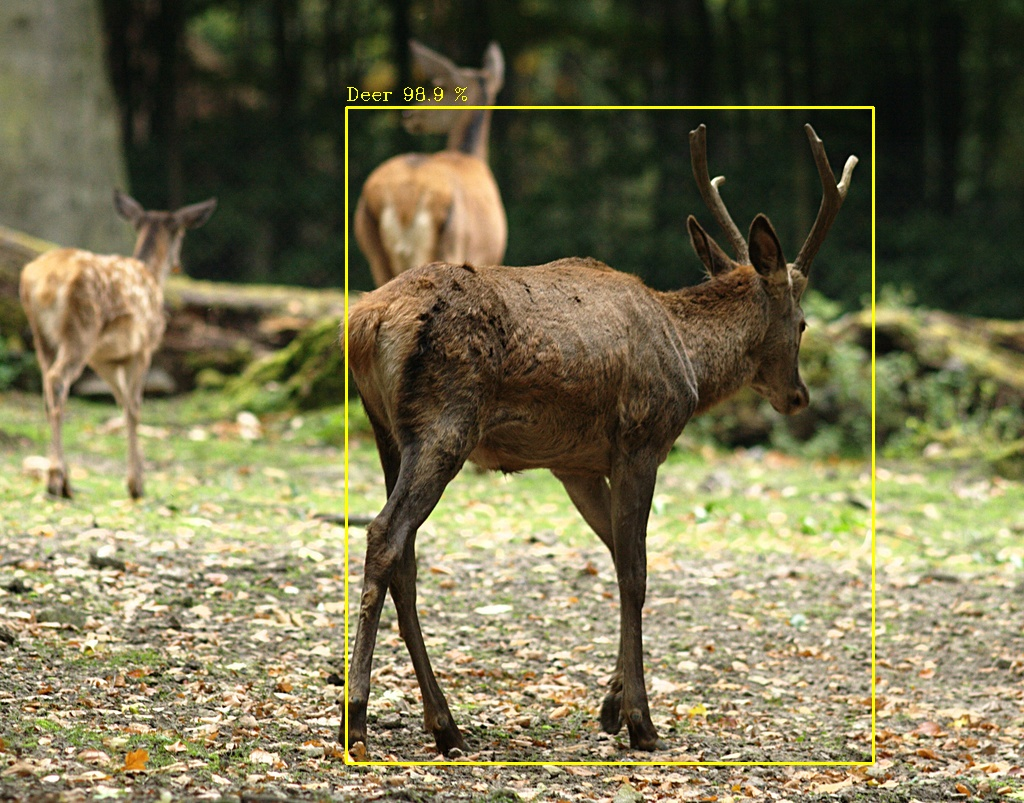
\includegraphics[width=0.9\textwidth]
  {model_compare_test__ssd_inception_v2.jpg}
  \captionof{figure}{Inferenzergebnis: SSD}
  \label{fig:infer_res_ssd}
\end{minipage}
\begin{minipage}{0.5\textwidth}
  \centering
  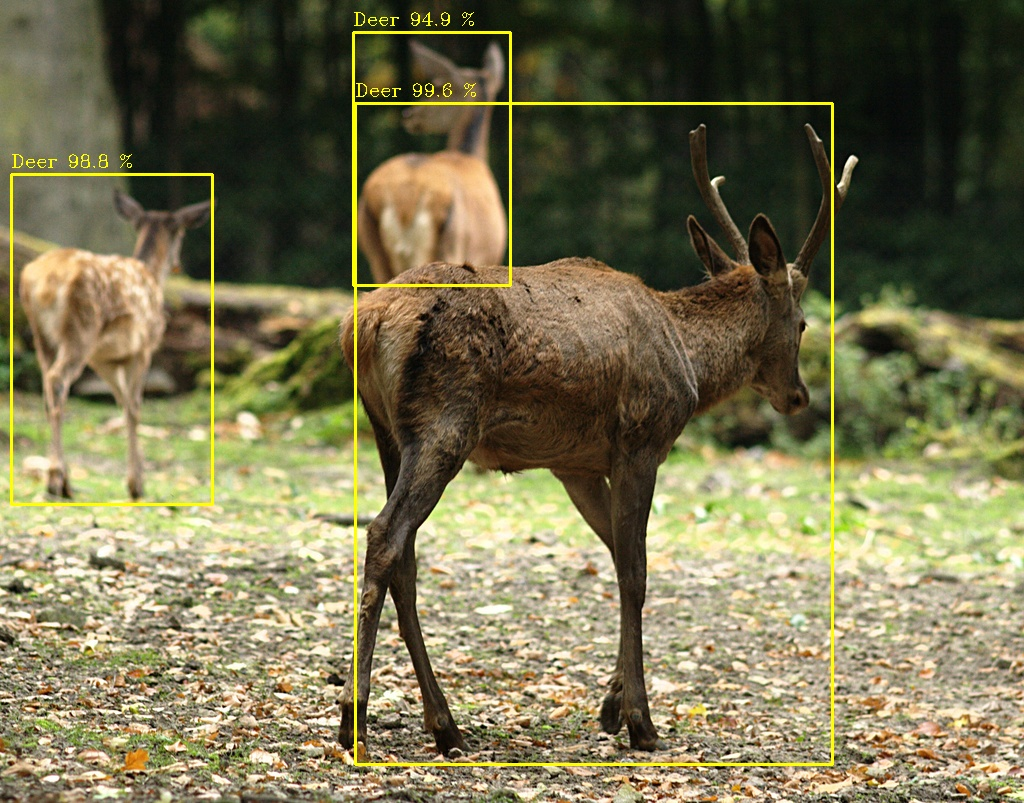
\includegraphics[width=0.9\textwidth]
  {model_compare_test__faster_rcnn_inception_v2_early_stopping.jpg}
  \captionof{figure}{Inferenzergebnis: Faster R-CNN}
  \label{fig:infer_res_faster_rcnn}
\end{minipage}


\subsubsection{Eigene Aufnahmen}

Bei der Inferenz auf die eigenen Bilder
war ein deutlicher Unterschied der Modelle festzustellen.

In aufsteigender Reihenfolge lieferten das SSD mit MobilenetV2,
das SSD mit InceptionV2, das Faster R-CNN mit 
Early Stopping und Faster R-CNN mit Augmentierten Daten
wie in den Abbildungen \ref{fig:infer_res_ssd_mobile}
bis \ref{fig:infer_rest_rcnn_aug} zu sehen ist, 
bessere Ergebnisse.

Auch hier fiel auf, dass Tiere, die weiter entfernt und 
damit kleiner abgebildet waren,
besser von den Faster R-CNN Modellen
erkannt wurden.

\vspace{1cm}
\begin{minipage}{0.5\textwidth}
  \centering
  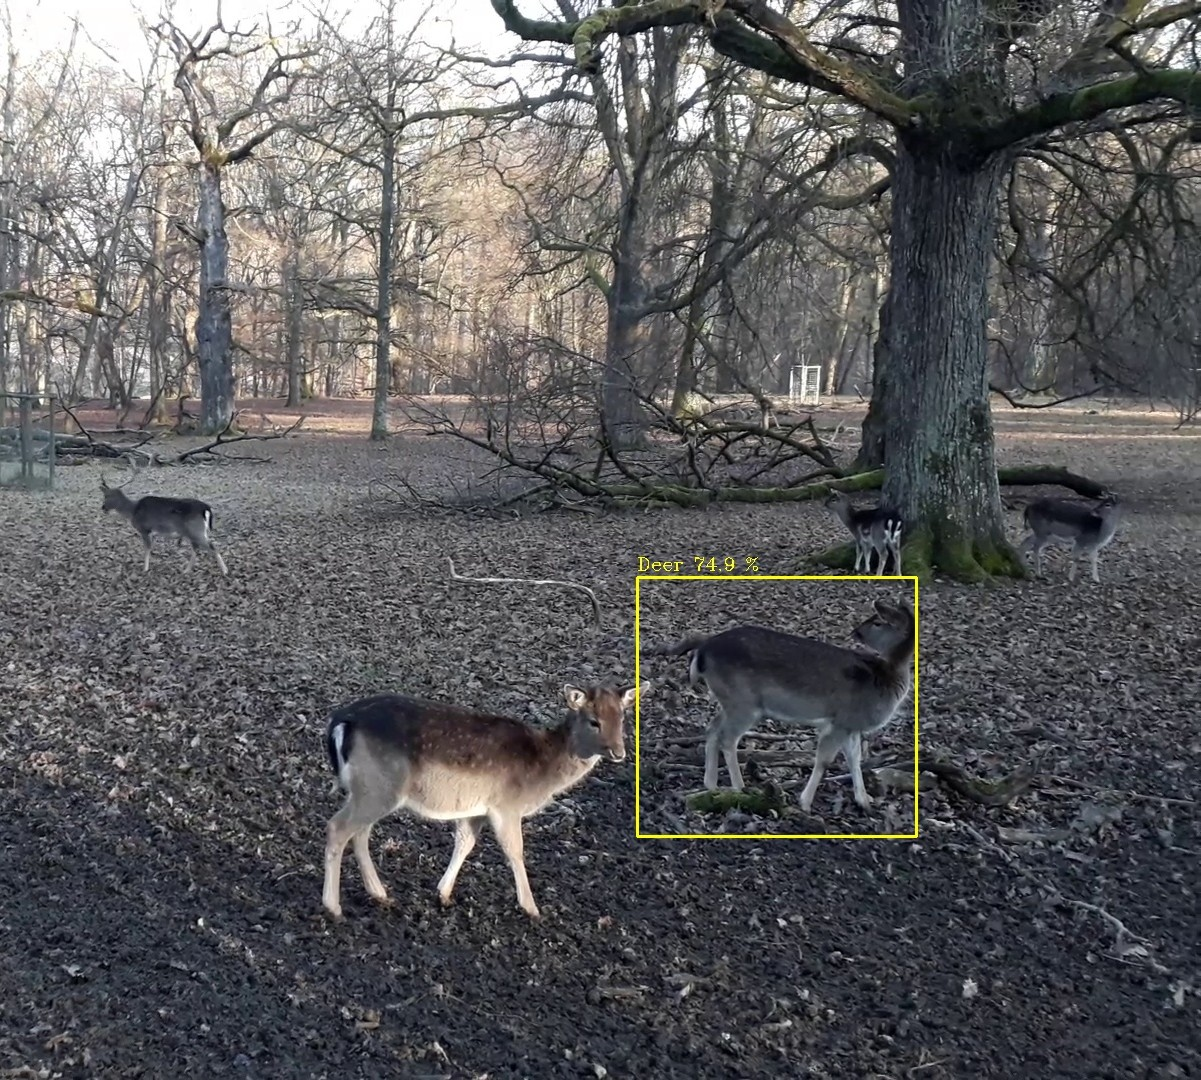
\includegraphics[width=0.9\textwidth]
  {model_compare_handy_ssd_mobilenet_v2.jpg}
  \captionof{figure}{Inferenzergebnis: SSD-Mobilnet}
  \label{fig:infer_res_ssd_mobile}
\end{minipage}
\begin{minipage}{0.5\textwidth}
  \centering
  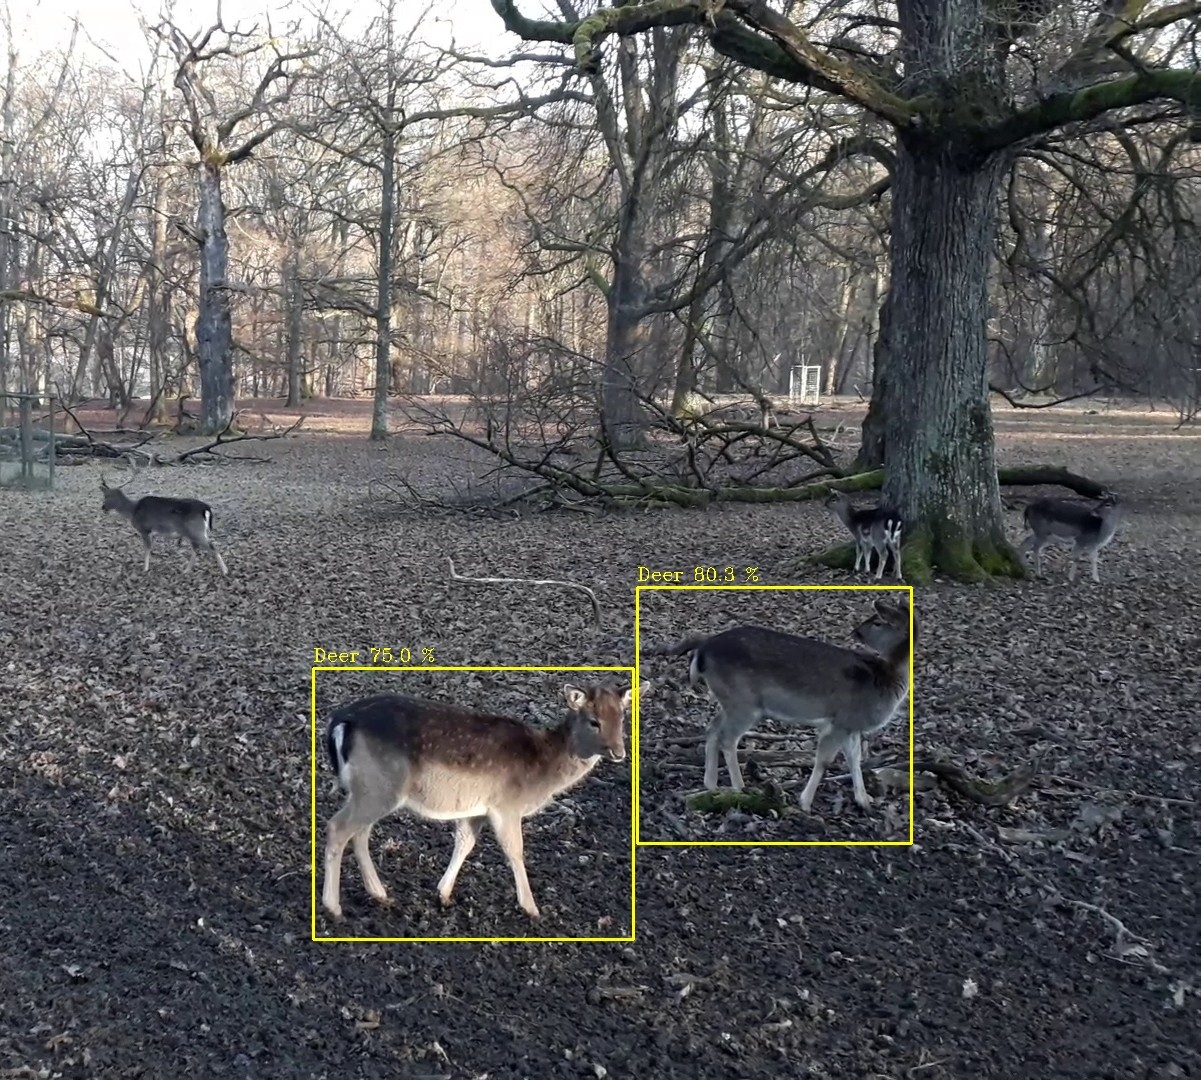
\includegraphics[width=0.9\textwidth]
  {model_compare_handy_ssd_inception_v2.jpg}
  \captionof{figure}{Inferenzergebnis: SSD-Inception}
  \label{fig:infer_res_ssd_inception}
\end{minipage}
\\[1cm]
\begin{minipage}{0.5\textwidth}
  \centering
  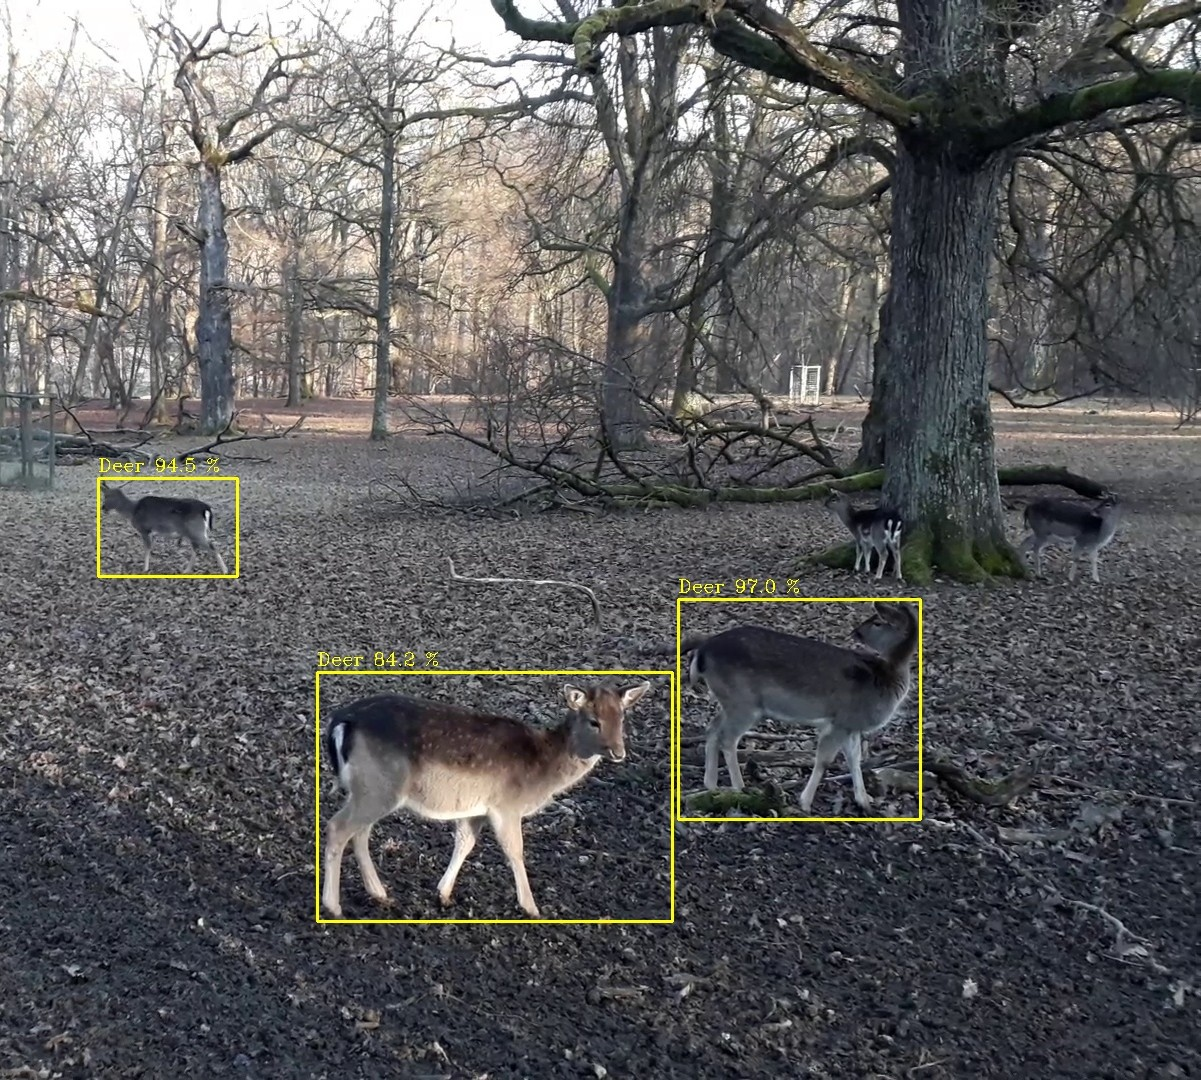
\includegraphics[width=0.9\textwidth]
  {model_compare_handy_faster_rcnn_inception_v2_early_stopping_ohne_aug.jpg}
  \captionof{figure}{Inferenzergebnis: Faster R-CNN\\mit Early Stopping}
  \label{fig:infer_res_rcnn_early_stopping}
\end{minipage}
\begin{minipage}{0.5\textwidth}
  \centering
  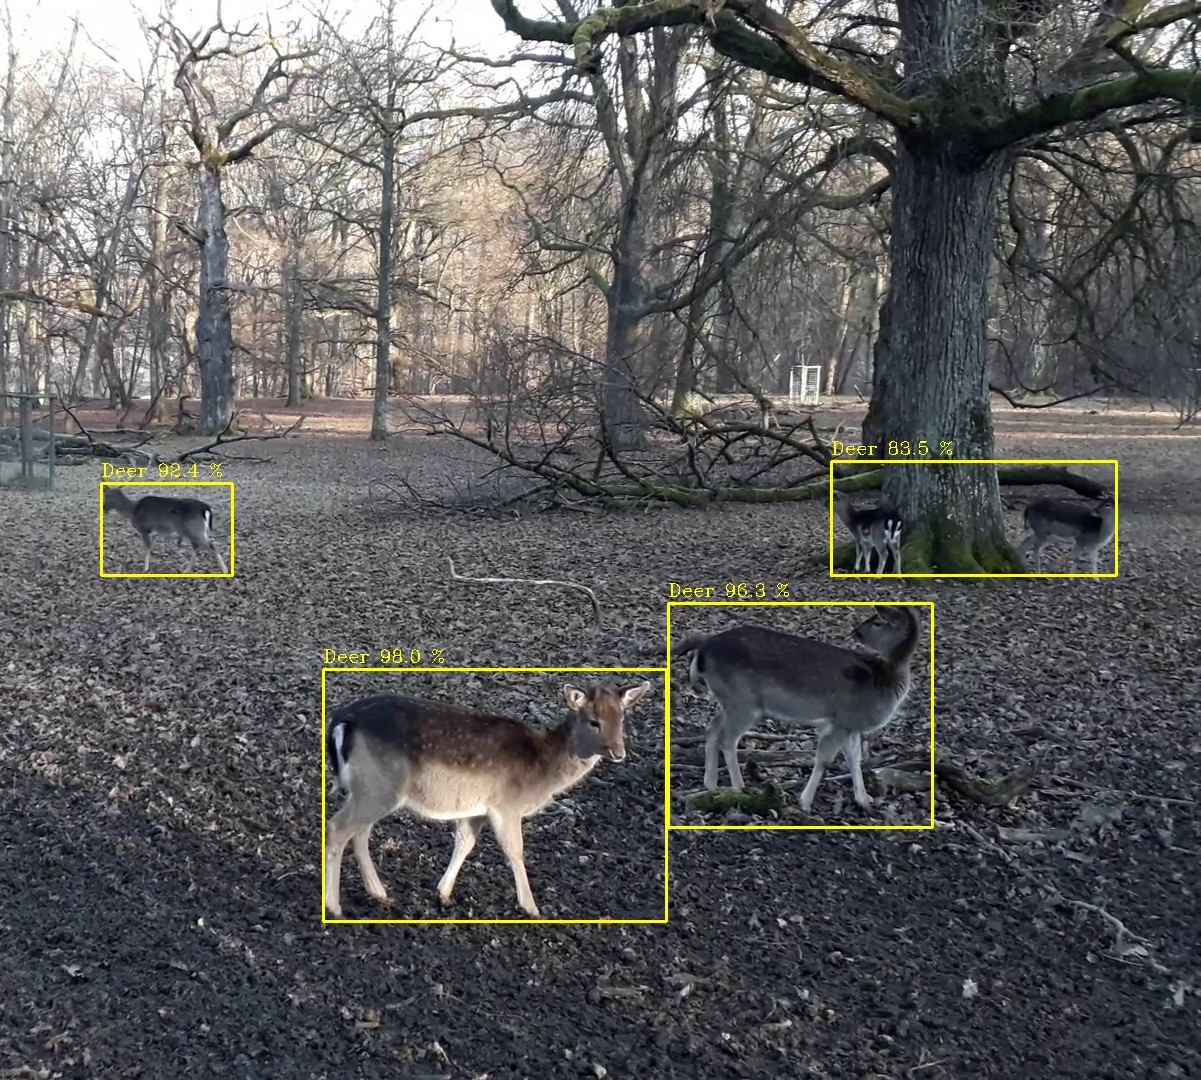
\includegraphics[width=0.9\textwidth]
  {model_compare_handy_faster_rcnn_inception_v2_early_stopping.jpg}
  \captionof{figure}{Inferenzergebnis: Faster R-CNN\\mit Augmentierung}
  \label{fig:infer_rest_rcnn_aug}
\end{minipage}



\subsubsection{iWildCam Datensatz}

Für die Test-Inferenz wurden die Klassen aus dem
\textit{iWildCam 2019 Dataset} heruntergeladen,
die sich mit den für das Training verwendeten Klassen
überschnitten.
Bei den Bildern des Datensatzes handelt es sich um Aufnahmen von
Wildtierkameras aus dem Süd- und Nordwesten Amerikas
welche aus der \textit{iNaturalist} und der \textit{Microsoft
DatAirSim} Datenbank stammen.


Darunter enthalten sind viele Nachtaufnahmen, welche teils 
schlecht beleuchtet und mit einer Infrarotkamera aufgenommen und daher 
in Graustufen sind.

Da die Inferenzergebnisse hier bei allen vier Modelvariationen 
nicht so gut wie bei den anderen Datensätzen waren, 
wurde versucht, eine Verbesserung der Inferenzergebnisse
durch weitere Optimierungen zu erreichen.


%----------------- SECTION: optimierung ---------------------
\section{Optimierungen: Faster R-CNN}
\label{sec:optimierung_faster_rcnn}

Als Ausgangslage zur Verbesserung der Ergebnisse diente 
das Faster R-CNN mit augmentiertem Datensatz, das bei 
den im vorherigen Abschnitt beschriebenen Evaluierungen 
die besten Resultate erzielte hatte.

Die Auswertung erfolgt hier wieder zunächst 
anhand der Evaluierungsmetriken und der Trainingsverläufe
aus \textit{TensorBoard} und anschließend anhand der
auf Testbilder ausgeführten Inferenzergebnisse.


\subsection{Verschiedene Augmentierungen}

Der erste Ansatz zur Verbesserung der Ergebnisse bestand darin,
das Faster R-CNN mit unterschiedlich starker Augmentierung
der Daten für insgesamt mehr Iterationen
(500k statt 200k) zu trainieren.

Dabei wurde wieder das im Abschnitt \ref{subsec:augmentation} 
erläuterte Augmentierungsverfahren angewendet, mit folgenden
zusätzlichen Variationen:

\begin{enumerate}
  \item Nur eine zufällige Augmentierung pro Bild, (anstelle von zwei)
  \item 4000 Bilder pro Klasse generieren (anstelle von 3000) 
\end{enumerate}

Die Trainingsergebnisse für 500k Iterationen sind anhand der 
Trainingsverläufe des Loss- und mAP-Wertes in den Abbildungen
\ref{plot:map_diff_aug} und \ref{plot:loss_diff_aug} dargestellt.
\vspace{1cm}

\begin{minipage}{0.5\textwidth}
  \centering
  \def\svgwidth{0.9\textwidth}
  \input{Bilder/plots/diff_aug_map.pdf_tex}
  \captionof{figure}{Trainingsverläufe: mAP}
  \label{plot:map_diff_aug}
\end{minipage}
\begin{minipage}{0.5\textwidth}
  \centering
  \def\svgwidth{0.9\textwidth}
  \input{Bilder/plots/diff_aug_loss.pdf_tex}
  \captionof{figure}{Trainingsverläufe: Loss}
  \label{plot:loss_diff_aug}
\end{minipage}

% Legende
% orange: FF7043
% blue  : 0077BB
% red   : CC3311
\begin{table}[htb]
  \centering
  \begin{tabular}{ m{0.4\textwidth}<{\centering}
                   m{0.2\textwidth}<{\centering}
                   m{0.2\textwidth}<{\centering}}
      $\color[HTML]{CC3311}\medbullet$ nur eine Augmentierung je Bild &
      $\color[HTML]{FF7043}\medbullet$  3000 Bilder &
      $\color[HTML]{0077BB}\medbullet$  4000 Bilder
  \end{tabular}    
\end{table}
\vspace{1cm}

Aufgrund des länger durchgeführten Trainings
ist bei allen Konfigurationen im Gegensatz zu den
Ergebnissen des vorherigen Abschnitts Overfitting 
festzustellen.

Wie zu erwarten war, fällt das Overfitting, bei den weniger  
augmentierten Datensätzen stärker aus, die jedoch andererseits
einen besseren mAP Wert erreichen konnten.


Ob sich, konkret für diesen Fall, ein höherer mAP oder 
besserer Loss Wert positiver auf das Ergebnis auswirkt,
konnte wieder mithilfe der Inferenz auf Testbilder 
herausgefunden werden.
\vspace{1cm}

\begin{minipage}{0.333\textwidth}
  \centering
  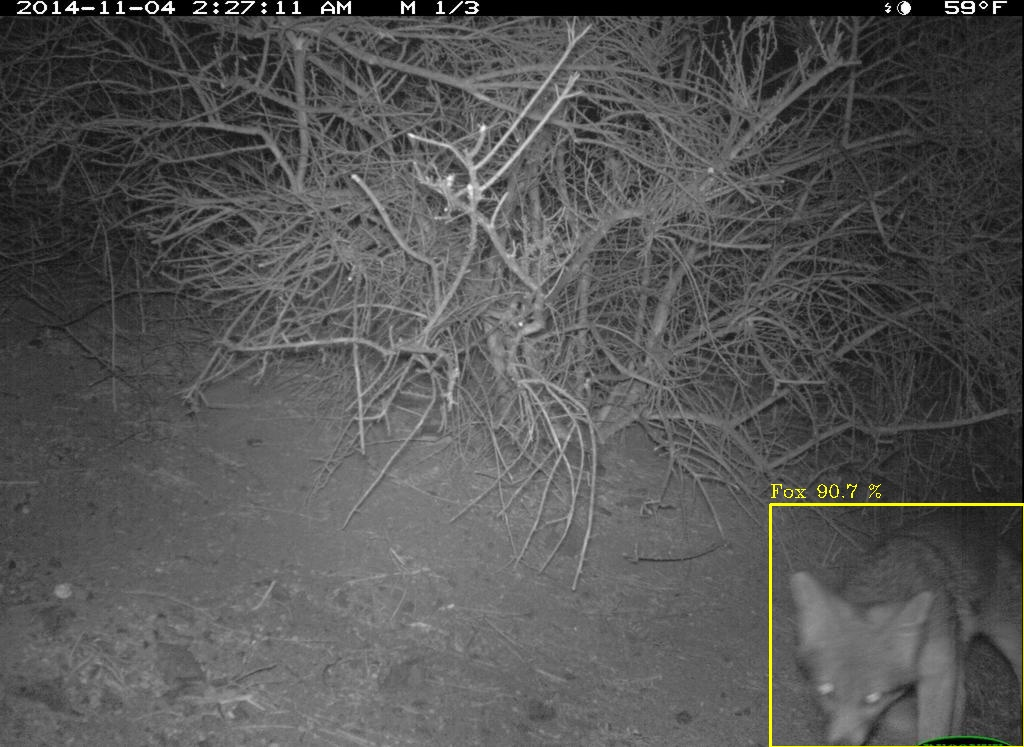
\includegraphics[width=\textwidth]{infer_images/iWildCam/fox/cut/59df5ee1-23d2-11e8-a6a3-ec086b02610b_faster_rcnn_inception_v2_3000.jpg}
  \captionof{figure}{Inferenz-\\ergebnis für 3000 Bilder}
  \label{fig:infer_res_3000}
\end{minipage}
\begin{minipage}{0.333\textwidth}
  \centering
  \label{fig:infer_res_4000}
  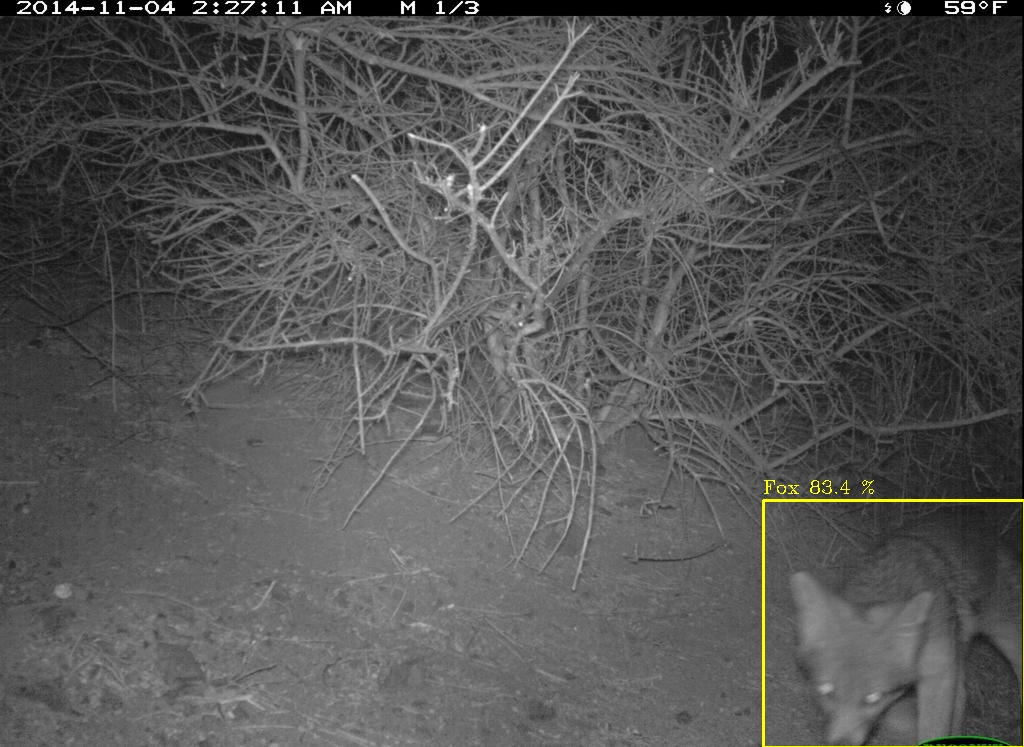
\includegraphics[width=\textwidth]{iWildCam/fox/cut/59df5ee1-23d2-11e8-a6a3-ec086b02610b_faster_rcnn_inception_v2_4000.jpg}
  \captionof{figure}{Inferenz-\\ergebnis für 4000 Bilder}
\end{minipage}
\begin{minipage}{0.333\textwidth}
  \centering
  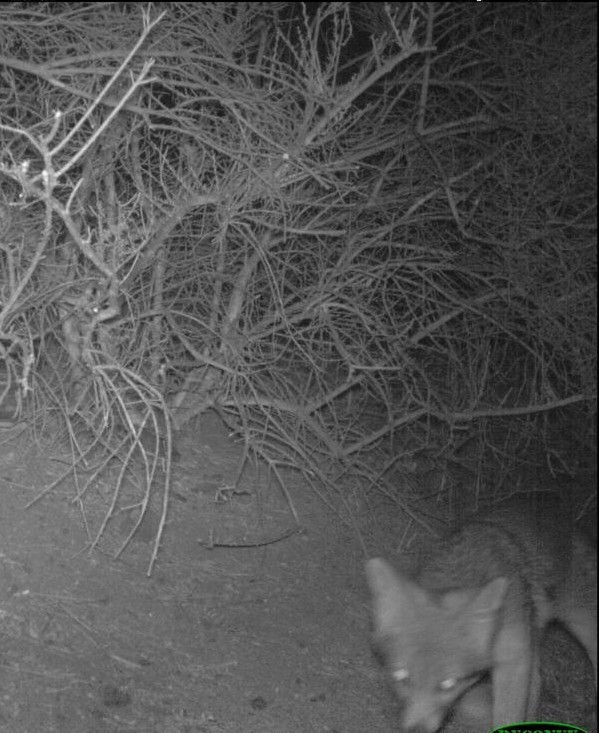
\includegraphics[width=\textwidth]{iWildCam/fox/cut/59df5ee1-23d2-11e8-a6a3-ec086b02610b_faster_rcnn_inception_v2_less_aug.jpg}
  \captionof{figure}{Inferenz-\\ergebnis für 50\% Augmentierung}
  \label{fig:infer_rest_05}
\end{minipage}
\vspace{1cm}

Die Abbildungen \ref{fig:infer_res_3000} bis \ref{fig:infer_rest_05}
zeigen beispielhaft die Inferenzergebnisse für Bilder des 
\textit{iWildCam} Datensatzes, bei dem sich dieses Mal der 
Unterschied deutlicher bemerkbar machte.
Bei den Modellen mit normaler oder mehr Augmentierung der 
Trainingsdaten war eine deutliche Verbesserung festzustellen, 
wohingegen das Modell, welches auf weniger stark augmentierte 
Daten trainiert wurde, die Tiere schlechter oder gar nicht erkannte.


\subsection{Verschiedene Regularisierungen}

Um das trotz Augmentierung zustandekommende \Gls{overfitting} zu 
vermeiden, wurde nun zusätzlich die \textit{L2 Regularisierung}
angewendet.
Diese soll, wie in dem Grundlagenkapitel (Abschnitt \ref{subsec:validation})
beschrieben wurde, durch Anhängen einer Aufsummierung der Gewichte
an die Loss-Funktion eine Überanpassung des Modells an die
Trainingsdaten reduzieren.

In der Konfigurationsdatei des Faster R-CNN kann dies
durch Setzten eines bestimmten Parameters sowohl für die
erste Stufe des Modells, dem \Gls{rpn},
als auch für die zweite Stufe, dem Klassifikationsmodell,
separat eingestellt werden.

Ebenso lassen sich die beiden Loss-Kurven, aus denen sich 
beim Faster R-CNN der gesamte Loss zusammensetzt,
separat anzeigen, was in den Verläufen der 
Abbildungen \ref{plot:aug_l2_classifier_loss}
und \ref{plot:aug_l2_rpn_loss} dargestellt ist.

Durch die getrennte Beobachtung der Loss-Kurven ließ sich 
feststellen, dass das \Gls{overfitting} nur das RPN betrifft,
weshalb der Parameter zur \textit{L2 Regulierung} nur 
für die erste Stufe eingestellt wurde.
Dafür wurde der Faktor $\lambda = 0.01$ gesetzt.

Vergleicht man nach dem Training mit 
reguliertem Modell wieder die Loss-Kurven, ist deutlich zu 
erkennen, dass sich das \Gls{overfitting} im RPN 
reduzieren ließ, wodurch sich auch der
in Abbildung \ref{plot:aug_l2_total_loss} 
dargestellte Gesamt-Loss verbesserte.

Die Verbesserung des Loss-Wertes 
ging hier wieder mit einer geringen 
Verschlechterung des mAPs einher, wie anhand der in Abbildung
\ref{plot:aug_l2_mAP} dargestellten Verläufe zu erkennen ist.

\vspace{1cm}
\begin{minipage}{0.5\textwidth}
  \centering
  \def\svgwidth{0.9\textwidth}
  \input{Bilder/plots/aug_l2_mAP.pdf_tex}
  \captionof{figure}{Trainingsverläufe: mAP}
  \label{plot:aug_l2_mAP}
\end{minipage}
\begin{minipage}{0.5\textwidth}
  \centering
  \def\svgwidth{0.9\textwidth}
  \input{Bilder/plots/aug_l2_total_loss.pdf_tex}
  \captionof{figure}{Trainingsverläufe: Gesamt-Loss}
  \label{plot:aug_l2_total_loss}
\end{minipage}
\\[1cm]
\begin{minipage}{0.5\textwidth}
  \centering
  \def\svgwidth{0.9\textwidth}
  \input{Bilder/plots/aug_l2_classifier_loss.pdf_tex}
  \captionof{figure}{Trainingsverläufe:\\Klassifikations-Loss}
  \label{plot:aug_l2_classifier_loss}
\end{minipage}
\begin{minipage}{0.5\textwidth}
  \centering
  \def\svgwidth{0.9\textwidth}
  \input{Bilder/plots/aug_l2_rpn_loss.pdf_tex}
  \captionof{figure}{Trainingsverläufe: RPN Loss}
  \label{plot:aug_l2_rpn_loss}
\end{minipage}
\begin{table}[htb]
  \centering
  \begin{tabular}{m{0.3\textwidth}<{\centering}
                  m{0.4\textwidth}<{\centering}}
     $\color[HTML]{CC3311}\medbullet$  nur Augmentierung &
     $\color[HTML]{0077BB}\medbullet$  Augmentierung + L2 Regularisierung
  \end{tabular}    
\end{table}
\vspace{1cm}

Zur Feststellung der Auswirkung 
der unterschiedlichen Ergebnisse wurde auch hier wieder die 
Testinferenz angewendet, was beispielhaft 
für Bilder der eigenen Aufnahmen in den 
Abbildungen \ref{fig:test_infer_normal_aug}
und \ref{fig:test_infer_aug_plus_l2} dargestellt ist.
\vspace{1cm}

\begin{minipage}{0.5\textwidth}
  \centering
  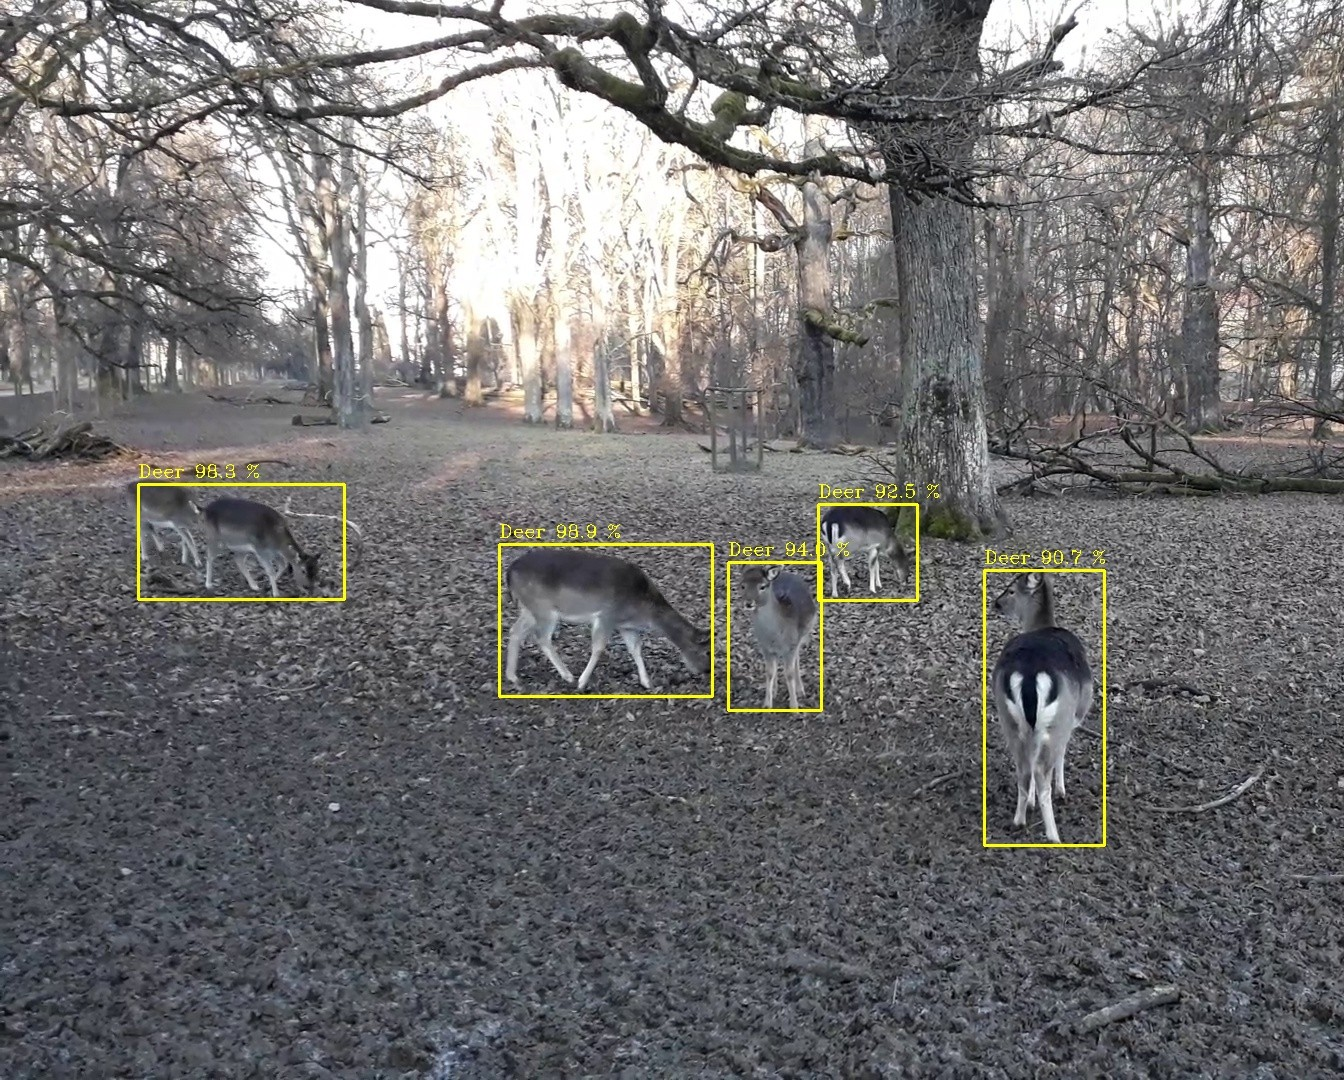
\includegraphics[width=0.95\textwidth]
  {eigene/20191229_145616_frame_20_faster_rcnn_inception_v2_3000.jpg}
  \captionof{figure}{Inferenzergebnis für\\
  reine Augmentierung}
  \label{fig:test_infer_normal_aug}
\end{minipage}
\begin{minipage}{0.5\textwidth}
  \centering
  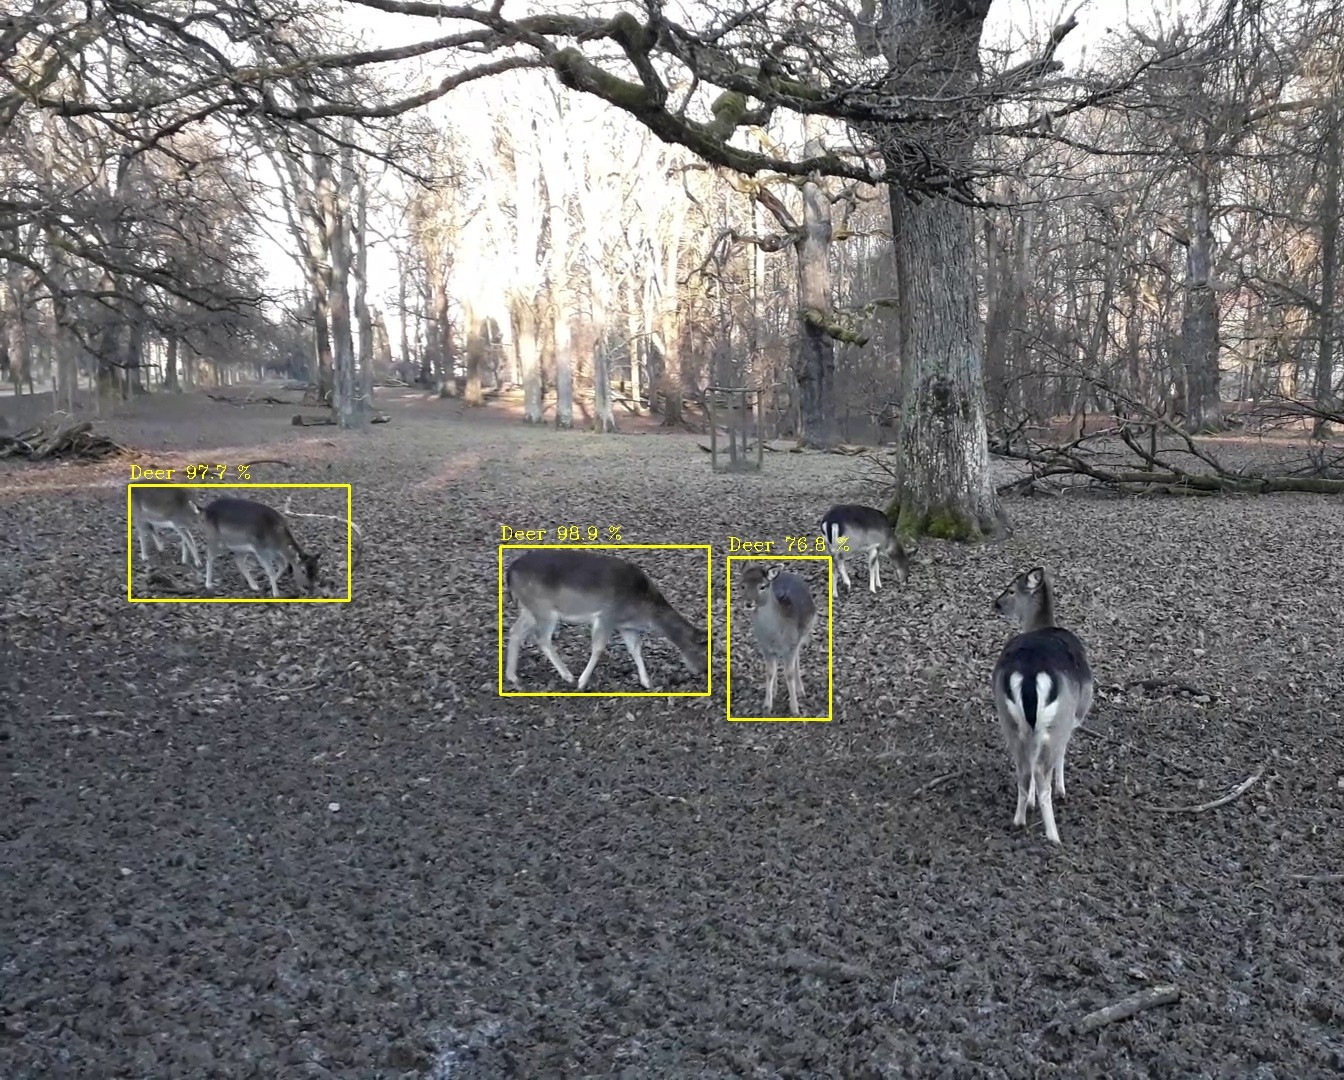
\includegraphics[width=0.95\textwidth]
  {eigene/20191229_145616_frame_20_faster_rcnn_inception_v2_l2.jpg}
  \captionof{figure}{Inferenzergebnis für\\
  Augmentierung und L2 Regularisierung}
  \label{fig:test_infer_aug_plus_l2}
\end{minipage}
\vspace{1cm}

Hier ergaben die Inferenzergebnisse, dass 
eine L2 Regulierung der Modelle
in den meisten Fällen keinen Einfluss auf das Ergebnis
hat, falls doch, dieses Ergebnis sich tendenziell sogar
verschlechterte.

Weitere angewendete Regularisierungen
waren \textit{Dropout} sowie L2 mit $\lambda = 0,02$.
Diese führten jedoch zu keiner nennenswerten Veränderung der
 Trainingsergebnisse und sind in Tabelle \ref{table:reg},
  zusammen mit den anderen Ergebnissen
 dargestellt.

\vspace{1cm}

\begin{table}[htb]
  \centering
  \begin{tabular}{m{0.35\textwidth}|m{0.25\textwidth}<{\centering}m{0.25\textwidth}<{\centering}}
  \hline
                    & mAP  & Loss  \\ \hline\hline
  Augmentierung (50\%) &  0,72    &    0,76   \\
   + L2 Reg. ($\lambda = 0,01$)            &   0,71     & 0,75       \\\hline
  Augmentierung (normal)     & 0,7  & 0,74            \\
  + Dropout          & 0,7  & 0,73            \\
  + L2 Reg. ($\lambda = 0,01$)    & 0,7  & 0,69            \\
  + L2 Reg. ($\lambda = 0,02$)    & 0,69 & 0,7             \\ \hline
  Augmentierung (4000 Samples) &0,7&0,71\\\hline
  \end{tabular}
  \caption{Trainingsergebnisse: Verschiedene Regularisierungstechniken}
  \label{table:reg}
\end{table}
\vspace{1cm}

Aus den Ergebnissen lässt sich schließen, dass die Art
der Aufbereitung der Daten den größeren Einfluss auf die Ergebnisse
haben und durch Anpassungen der Hyperparameter, wenn überhaupt,
nur noch geringfügige Optimierungen betrieben werden können.
So hat insgesamt das Faster R-CNN mit 500k Trainingsiterationen 
auf augmentierte Daten mit 3000 Bildern je Klasse, zu
den besten Ergebnissen bezüglich Genauigkeit geführt.


\section{Inferenzzeit}\label{sec:infertime}

Neben der Genauigkeit war die Ausführungszeit, welche ein Modell
für die Inferenz benötigt, ein weiteres Kriterium für die Auswahl
des in der Anwendung zu verwendenden Modells.
Einer der Faktoren, der die Inferenzzeit beeinflusst,
ist die Art Hardware, auf der die Inferenz stattfindet,
sowie die zur Implementierung verwendete \textit{Library}.

Die Hardware war mit dem \textit{Neural Compute Stick 2}
festgelegt, als \textit{Library} kamen dafür \textit{OpenCV}
oder \textit{OpenVino} in Frage, wobei mit
\textit{OpenVino} die Möglichkeit 
zur asynchronen Inferenzausführung, sowie der Verwendung mehrerer,
parallel ausgeführter Inferenz-Requests besteht,
wodurch sich die Inferenzzeit optimieren lässt.

Ein weiterer Faktor ist die Komplexität des \Glspl{cnn}, sowie die 
für die Objekterkennung verwendete Modellarchitektur.
Üblicherweise sind komplexere Modelle wie das Faster R-CNN
zwar genauer, dafür auch langsamer.

Um den Effekt, den die drei unterschiedlichen
für das Training verwendeten Varianten SSD mit MobilenetV2, 
SSD mit InceptionV2 und Faster R-CNN mit InceptionV2 auf die
Inferenzzeit haben zu untersuchen
wurden diese durch Messen der Inferenzzeit verglichen.

Dabei wurde die asynchrone Inferenz mit unterschiedlicher Anzahl 
an Inferenz-Requests verwendet.
Im Folgenden Abschnitt wird zunächst die Funktionsweise der synchronen und asynchronen
Inferenzausfürung mit \textit{OpenVino} erklärt.



\subsection{Synchrone und asynchrone Inferenz}

Wird die Inferenz im synchronen Modus ausgeführt, kann immer
nur entweder inferiert werden, oder das Vor- und 
Nachverarbeiten der Bilder stattfinden.

Die Vorverarbeitung der Bilder beeinhaltet dabei
zum Beispiel die Umwandlung des von der Kamera gelieferten 
Bildformats in das für das jeweilige Modell richtige 
Input Format.
Die Nachverarbeitung bezieht sich auf das Verwenden 
der Inferenzergebnisse in der Anwendung.

Die Implementierung der Inferenz in \textit{OpenVino} erfolgt
dementsprechend sequentiell, wie im Algorithmus
\ref{code:sync} als Pseudocode dargestellt ist.

Anhand des zeitlichen Ablaufs, dargestellt in Abbildung
\ref{fig:sync}, sind die Abschnitte in denen
keine Inferenz stattfinden kann zu erkennen.

\vspace{1cm}
\begin{minipage}{0.1\textwidth}
  \hfill
\end{minipage}
\begin{minipage}{0.5\textwidth}
  \begin{algorithm}[H]
    \caption{Synchrone Inferenz}
    \label{code:sync}
    \begin{algorithmic}
    \WHILE{\TRUE}
        \STATE capture FRAME
        \STATE preprocess CURRENT InferRequest
        \STATE \textbf{start} CURRENT InferRequest
        \STATE \textbf{wait} for CURRENT InferRequest
        \STATE process CURRENT result
    \ENDWHILE
    \end{algorithmic}
  \end{algorithm}  
\end{minipage}
\begin{minipage}{0.4\textwidth}
  \centering
  \vspace{1cm}
  \def\svgwidth{0.5\textwidth}
  \input{Bilder/sy_asy_legend.pdf_tex}
\end{minipage}

\vspace{1cm}
\begin{figure}[H]
  \centering
  \def\svgwidth{0.9\textwidth}
  %\tikzset{
    desicion/.style={
        diamond,
        draw,
        text width=4em,
        text badly centered,
        inner sep=0pt
    },
    block/.style={
        rectangle,
        draw,
        text width=5em,
        text height=1em,
        text centered
    },
    arrow/.style={
        draw,
        >=latex,
        ->
    }
}


\begin{tikzpicture}

    \node(infer1) [block] {infer1};
    \draw[arrow] (0,-1em) -- (10,-1em);
    % \node (A) [desicion] {entschei\\dung};
    % \node (B) [block, below of=A, node distance=5cm, text width=5em] {bock};
    % \node (C) [block, right of=A, node distance=5cm] {noch ein\\bock};


    % \draw[arrow] (A) --  node [left, fill=white] {yes} (B);
    % \draw[arrow] (A) -- node [below, near end] {crap} (C); 
    % \draw[arrow] (B) -| node [near start, fill=white] {yes} (C);

\end{tikzpicture}

  \input{Bilder/sync_infer.pdf_tex}
  \caption{Zeitlicher Ablauf der synchronen Inferenz}
  \label{fig:sync}
\end{figure}


Da die Inferenz auf dem \textit{Myriad Chip} des NCS2
und nicht auf dem ausführenden PC bzw. \textit{Raspberry Pi} läuft,
kann diese ungehindert, parallel zum restlichen Programmablauf, 
erfolgen.

In \textit{OpenVino} wird dieser Ablauf mithilfe
 der \textit{Asynchronen \Gls{api}}
erreicht, die über einen bestimmten Funktionsaufruf
die Inferenz in einem seperaten \Gls{thread} startet.

Indem vor Erhalt und Verarbeitung eines aktuellen 
Inferenzergebnisses der Inferenz-Request für
den nächsten Durchlauf aufgegeben wird, wie im Algorithmus
\ref{code:async} als Pseudocode dargestellt, kann der in
Abbildung \ref{fig:async} dargestellte zeitliche Ablauf
erreicht werden.
\vspace{1cm}

\begin{minipage}{0.1\textwidth}
  \hfill
\end{minipage}
\begin{minipage}{0.5\textwidth}
  \begin{algorithm}[H]
    \caption{Asynchrone Inferenz}
    \label{code:async}
    \begin{algorithmic}
    \WHILE{\TRUE}
        \STATE capture FRAME
        \STATE preprocess NEXT InferRequest
        \STATE \textbf{start} NEXT InferRequest
          \STATE \textbf{wait} for CURRENT InferRequest
          \STATE process CURRENT result
          \STATE swap CURRENT and NEXT InferRequest
    \ENDWHILE
    \end{algorithmic}
  \end{algorithm}
\end{minipage}
\begin{minipage}{0.4\textwidth}
  \centering
  \vspace{1cm}
  \def\svgwidth{0.5\textwidth}
  \input{Bilder/sy_asy_legend.pdf_tex}
\end{minipage}

\vspace{1cm}

\begin{figure}[H]
  \centering
  \def\svgwidth{0.9\textwidth}
  \input{Bilder/async_infer.pdf_tex}
  \caption{Zeitlicher Ablauf der asynchronen Inferenz}
  \label{fig:async}
\end{figure}

Die hier mit \textit{Current} und \textit{Next} bezeichneten 
Inferenz-Requests stehen für die Indizes der jeweiligen Requests
und können beliebig erweitert werden. 
Dadurch wird erreicht, dass die Inferenz auf mehreren \Glspl{thread} 
parallel ausgeführt wird.


\subsection{Vergleich der Modelle}

Mithilfe eines Python Scripts, in welchem die asynchrone Inferenz 
für eine variabel einstellbare Anzahl an Inferenz Requests
implementiert wurde, konnte für die drei Modelle die 
durchschnittliche Anzahl der Bilder die pro Sekunde inferiert
werden können (\Gls{fps}) der Inferenz ermittelt werden.

Diese wurden auf dem \textit{Raspberry Pi} mit dem \textit{Neural Compute Stick} 
ausgeführt und lieferten die in Tabelle \ref{table:infertime}
dargestellten Ergebnisse.

\vspace{1cm}
\begin{table}[H]
  \centering
  \begin{tabular}{m{0.25\textwidth}|m{0.1\textwidth}<{\centering}|m{0.1\textwidth}<{\centering}|m{0.1\textwidth}<{\centering}|m{0.1\textwidth}<{\centering}}
  \hline
  \multirow{2}{*}{Model} & \multicolumn{4}{c}{Asynchrone Inferenz-Requests} \\ \cline{2-5} 
                         & 1           & 2          & 3          & 4          \\ \hline\hline
  SSD MobilenetV2        & 19,5           & 35,2          & 40,6          & 40,3          \\
  SSD InceptionV2        & 15,6           & 27,7          & 31,1          & 31,7          \\
  Faster R-CNN Incept.   & 0,63           & 0,67          & 0,75          & 0,74          \\ \hline
  \end{tabular}
  \caption{Vergleich von Inferenzzeiten der Modelle in FPS}
  \label{table:infertime}
\end{table}
\vspace{1cm}

Die asynchrone Inferenzausführung führte bei allen Modellen 
für bis zu drei Inferenz-Requests, zu besseren Ergebnissen.
Ein deutlicher Unterschied der Inferenzzeit war 
zwischen SSD und Faster-R-CNN-Architekturen festzustellen.

Da für die Anwendung zur Wildtiererkennung 
keine Realtime-Performance erforderlich ist,
wurde durch geschickte Implementierung der Inferenz in der 
Applikation, trotz langsamerer Inferenzzeit, das 
Faster R-CNN verwendet.
